% !TEX root = pfc.tex

O método proposto foi implementado em forma de um \textit{software} multiplataforma, desenvolvido em linguagem \verb!C++! \citep{cplusplus:2013:online}, com intuito de obter um bom desempenho de execução e fácil implementação utilizando os conceitos de programação orientada a objetos.

Como biblioteca para processamento das imagens, foi utilizado a OpenCV 2.4.4 \citep{opencv_library}, contribuindo para que operações complexas de visão computacional pudessem ser realizadas com poucas linhas de código. O desenvolvimento do método não está preso à tecnologia escolhida, podendo ser empregado utilizando outras linguagens de programação, bem como outras bibliotecas. A tecnologia foi escolhida visando a simplicidade no processo de desenvolvimento das operações de processamento de imagens, que estão bem detalhadas pelos trechos de código na Seção \ref{sec:fluxo_de_processos}.

\section{Testes} % (fold)
\label{sec:testes}

Todos os vídeos foram capturados por um aparelho celular Samsung OMNIA W GT-I8350 \citep{omnia:2013:online}, como descrito na Seção \ref{sec:caracter_sticas_de_captura}. As imagens foram feitas na passarela localizada na Av. Presidente Carlos Luz, nos dois sentidos da via, como ilustra a Figura \ref{fig:sentidos}. Duas configurações de captura foram utilizadas:

\begin{itemize}
  \item HD 720p: gerando vídeos com resolução $1280\times 720$, e \textit{framerate} de 29 FPS;
  \item VGA: gerando vídeos com resolução $640\times 480$, e \textit{framerate} de 29 FPS.
\end{itemize}

Com intuito de equiparar as resoluções dos vídeos gerados a partir das duas configurações de captura, as amostras em HD foram redimensionadas para ter altura e largura metade do valor original, resultando em vídeos com resolução $640\times 360$. A Tabela \ref{tab:videos_teste} lista as amostras utilizadas.

% \noindent Uma terceira resolução foi obtida a partir dos vídeos em HD, aplicando uma operação para redimensioná-los com altura e largura a metade do valor original. Essas variações de cena e resolução foram feitas com o objetivo de avaliar o comportamento do método em diferentes condições. Assim, será possível identificar o impacto de cada variável no resultado final. A Tabela \ref{tab:videos_teste} lista as amostras utilizadas.

\begin{figure}[ht]
  \begin{center}
    \begin{subfigure}[b]{.49\textwidth}
      \begin{center}
        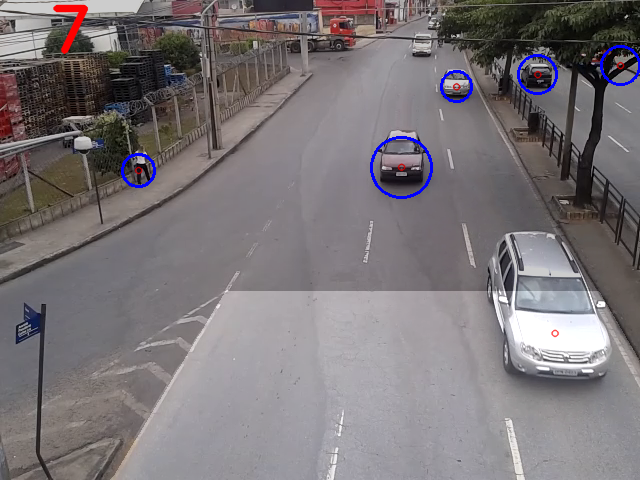
\includegraphics[width=1\linewidth]{imgs/trackers.png}
      \end{center}
      \caption{}
      \label{fig:sentido_pampulha}
    \end{subfigure}
    \begin{subfigure}[b]{.49\textwidth}
      \begin{center}
        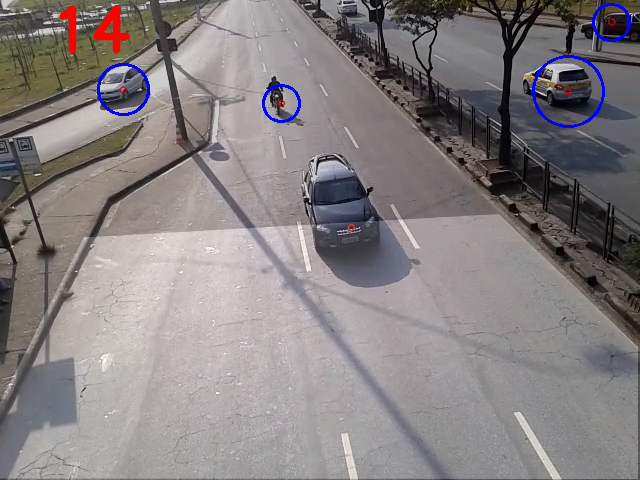
\includegraphics[width=1\linewidth]{imgs/sentido_centro.png}
      \end{center}
      \caption{}
      \label{fig:sentido_centro}
    \end{subfigure}
  \end{center}
  \caption{Resultado do método de contagem para dois tipos de cena. (a) Av. Carlos Luz, sentido Pampulha; (b) Av. Carlos Luz, sentido Centro.}
  \label{fig:sentidos}
\end{figure}

\begin{table}[ht]
  \caption{Vídeos utilizados nos testes.}
  \label{tab:videos_teste}
  \begin{center}
    \begin{tabular}{clcccc}
    \toprule
    \textbf{Nº} & \textbf{Nome do vídeo} & \textbf{Resolução} & \textbf{Duração} & \textbf{FPS} \\
    \midrule
      1 & carlos\_luz\_centro\_vga & $ 640\times 480 $ & 00:05:23 & 29 \\
      2 & carlos\_luz\_centro\_hd\_resized & $ 640\times 360 $ & 00:05:25 & 29 \\
      % carlos\_luz\_centro\_hd & $ 1280\times 720 $ & 00:05:29 & 29 \\
      3 & carlos\_luz\_pampulha\_vga\_1 & $ 640\times 480 $ & 00:05:43 & 29 \\
      4 & carlos\_luz\_pampulha\_vga\_2 & $ 640\times 480 $ & 00:05:19 & 29 \\
      5 & carlos\_luz\_pampulha\_hd\_2\_resized & $ 640\times 360 $ & 00:06:19 & 29 \\
      % carlos\_luz\_pampulha\_hd\_2 & $ 1280\times 720 $ & 00:06:21 & 29 \\
    \bottomrule
    \end{tabular}
  \end{center}
\end{table}

Tanto o desenvolvimento do \textit{software}, quanto os testes, foram feitos em um \textit{Laptop} Dell Vostro V131, Processador Intel Core I3-2330M (2.20GHZ, dual core 4 Threads, 3MB L3 cache), 8GB de memória RAM, em ambiente Arch Linux.

% section testes (end)

\section{Resultados e discussão} % (fold)
\label{sec:resultados_e_discuss_o}

As cinco amostras listadas na Tabela \ref{tab:videos_teste} foram analisadas e cada um dos elementos da matriz de confusão (VP, VN, FP e FN) foram identificados e quantificados, segundo o método de análise de desempenho definido na Seção \ref{sec:avalia_o_dos_resultados}. Foram utilizados exatos $6000$ \textit{frames} de cada amostra de vídeo (cerca de 3 minutos e 20 segundos) para a construção da matriz. A Tabela \ref{tab:matrix_result} mostra o resultado da contagem dos eventos da matriz de confusão e os índices de desempenho calculados a partir deles, incluindo o índice Kappa (K).

\begin{table}[ht]
  \caption{Resultado obtido da contagem nas amostras de teste, índices de desempenho e índice Kappa (K).}
  \label{tab:matrix_result}
  \begin{center}
    \begin{tabular}{c|cccc|cccccc|cc}
    \toprule
    \textbf{Nº} & \textbf{VP} & \textbf{VN} & \textbf{FP} & \textbf{FN} & \textbf{E} & \textbf{VPN} & \textbf{P} & \textbf{R} & \textbf{FM} & \textbf{A} & \textbf{K} & \textbf{Qual.} \\
    \midrule
      1 & 92 & 35 & 2 & 6 & 0.95 & 0.85 & 0.98 & 0.94 & 0.96 & 0.94 & 0.86 & Excelente\\
      2 & 76 & 34 & 6 & 10 & 0.85 & 0.77 & 0.93 & 0.88 & 0.90 & 0.87 & 0.71 & Muito bom\\
      3 & 107 & 19 & 1 & 26 & 0.95 & 0.42 & 0.99 & 0.80 & 0.89 & 0.82 & 0.49 & Bom \\
      4 & 87 & 28 & 8 & 22 & 0.78 & 0.56 & 0.92 & 0.80 & 0.85 & 0.79 & 0.51 & Bom \\
      5 & 94 & 37 & 2 & 15 & 0.95 & 0.71 & 0.98 & 0.86 & 0.92 & 0.89 & 0.73 & Muito bom\\
    \bottomrule
    \end{tabular}
  \end{center}
\end{table}

Pode-se observar que em todas as amostras o índice referente à Precisão foi superior a $0.92$. Esse resultado pode ser comprovado pela baixa quantidade de eventos do tipo falso positivo FP na matriz de confusão, ou seja, poucos objetos foram contabilizados como veículos quando na realidade não eram. Isso acontece graças ao algoritmo de rastreamento e contagem proposto na Subseção \ref{sub:rastreamento_e_contagem}, que através de \textit{trackers}, \textit{keypoints} e uma região de contagem garante o correto rastreio dos objetos em movimento, contabilizando apenas os veículos pertencentes ao sentido da via. 

Nas amostras 1 e 2, que são imagens da Av. Carlos Luz no sentido Centro, a qualidade ficou entre muito bom e excelente, segundo escala definida na Tabela \ref{tab:indice_kappa}; já  nas amostras 3, 4 e 5, que se referem à mesma via no sentido Pampulha, a qualidade ficou entre bom e muito bom. Essa variação na qualidade da classificação acontece principalmente pelas características do tráfego de cada sentido da via. 

Analisando os vídeos é possível identificar vários veículos de grande porte trafegando no sentido Pampulha, como mostra a Figura \ref{fig:veiculo_grande}, muitos saindo da Fábrica da Coca-Cola ali localizada, contrariando as premissas previamente definidas na Seção \ref{sec:caracter_sticas_de_captura}. Esse tipo de tráfego gera vibrações na câmera e oclusões, comprometendo os processos de subtração de \textit{background} e detecção de \textit{blobs} (Figuras \ref{fig:problema_veiculo_grande} e \ref{fig:problema_veiculo_junto}, respectivamente). Esses problemas podem ser constatados no aumento do número de eventos do tipo falso negativo FN, ou seja, veículos que não são contabilizados quando deveriam ser, contribuindo para que índices de desempenho como Acurácia e Kappa piorem.

Os eventos falso positivo FP podem ser percebidos quando existe vibrações e movimentação da câmera. A Figura \ref{fig:camera_moveu} ilustra esse fenômeno através das falhas de detecção, criando \textit{keypoints} sobre regiões que não representam veículos em movimento.

\begin{figure}[ht]
  \begin{center}
    \begin{subfigure}[b]{.49\textwidth}
      \begin{center}
        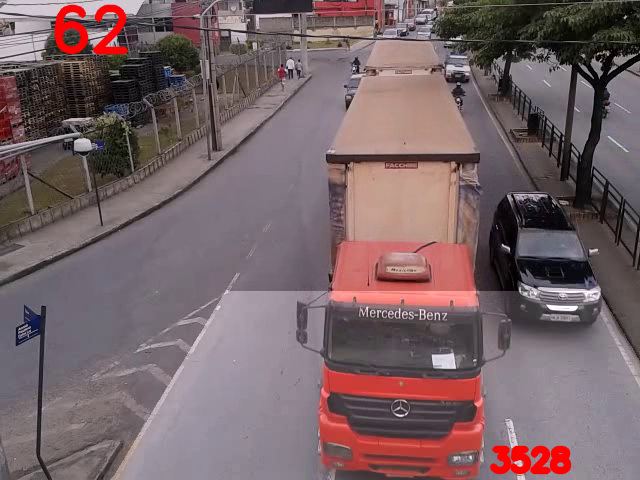
\includegraphics[width=1\linewidth]{imgs/veiculo_grande.png}
      \end{center}
      \caption{}
      \label{fig:veiculo_grande}
    \end{subfigure}
    \begin{subfigure}[b]{.49\textwidth}
      \begin{center}
        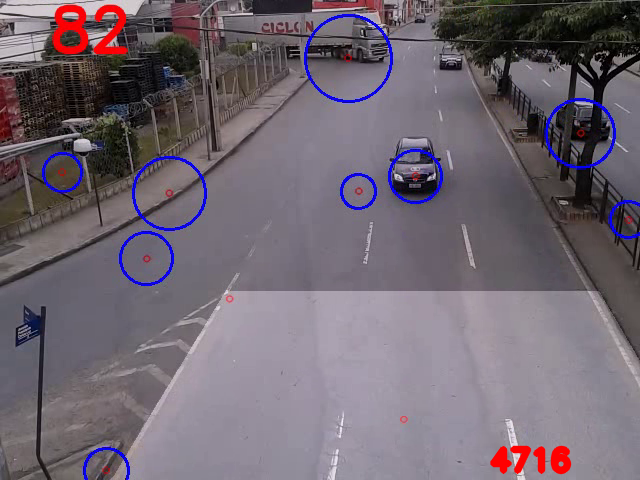
\includegraphics[width=1\linewidth]{imgs/camera_moveu.png}
      \end{center}
      \caption{}
      \label{fig:camera_moveu}
    \end{subfigure}
  \end{center}
  \caption{Tipo de tráfego encontrado nas vias. (a) Veículos muito grandes causam problemas como oclusão e vibrações na passarela. (b) Falsas detecções de veículos quando a câmera sofre movimentação.}
  \label{fig:tipo_de_trafego}
\end{figure}

\begin{figure}[ht]
  \begin{center}
    \begin{subfigure}[b]{.49\textwidth}
      \begin{center}
        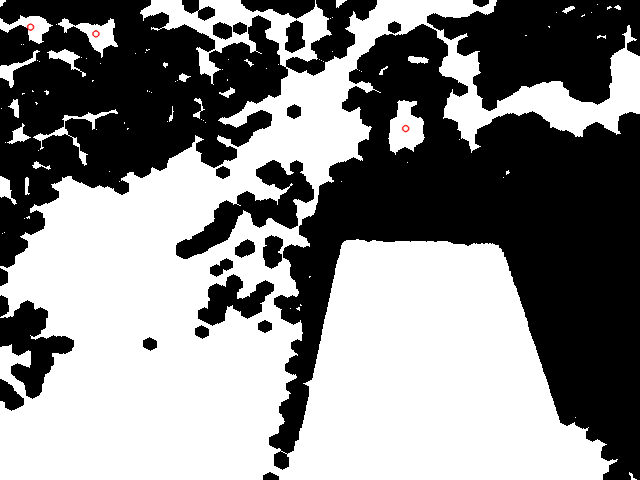
\includegraphics[width=1\linewidth]{imgs/problema_veiculo_grande.png}
      \end{center}
      \caption{}
      \label{fig:problema_veiculo_grande}
    \end{subfigure}
    \begin{subfigure}[b]{.49\textwidth}
      \begin{center}
        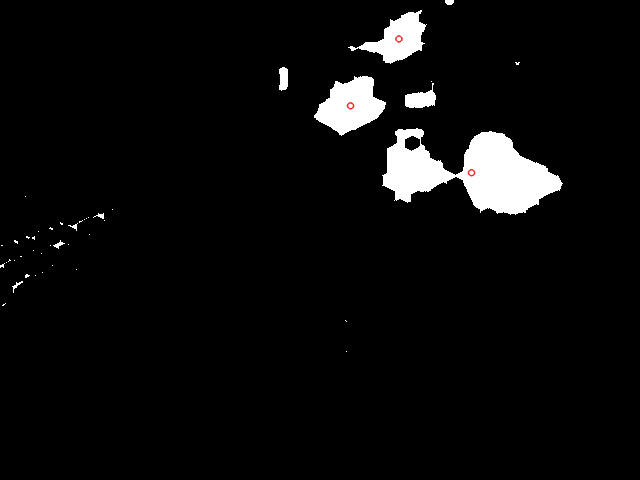
\includegraphics[width=1\linewidth]{imgs/problema_veiculo_junto.png}
      \end{center}
      \caption{}
      \label{fig:problema_veiculo_junto}
    \end{subfigure}
  \end{center}
  \caption{Problemas encontrados no processamento de imagens. (a) A operação de subtração de \textit{background} fica comprometida quando veículos com área muito grande aparecem na cena e causam vibração na câmera. (b) Veículos próximos ou em oclusão são detectados como um único objeto, gerando eventos falso negativo FN.}
  \label{fig:problemas}
\end{figure}

% section resultados_e_discuss_o (end)

% \section{Resultados finais} % (fold)
% \label{sec:resultados_finais}


% Na Tabela \ref{tab:resultados_contagem} são apresentados os resultados obtidos pela contagem via métodos manual e automático, indicando o percentual de acerto para cada amostra. É importante destacar que o resultado da contagem automática representa o total de veículos identificados na amostra, incluindo falsos positivos e descartando objetos detectados ou rastreados incorretamente. Portanto, os percentuais de acerto são medições estatísticas, que representam apenas o desvio existente entre o valor real e o valor medido.

% \begin{table}[ht]
%   \caption{Resultados de contagem volumétrica.}
%   \label{tab:resultados_contagem}
%   \begin{center}
%     \begin{tabular}{l|cccc}
%     \toprule
%     \textbf{Nome do vídeo} & \textbf{Resolução} & \textbf{Manual} & \textbf{Autom.} & \textbf{\% acerto}\\
%     \midrule
%       carlos\_luz\_centro\_vga & $ 640\times 480 $ & 164 & 156 & 95,12 \\
%       carlos\_luz\_centro\_hd\_resized & $ 640\times 360 $ & 150 & 153 & 98,04 \\
%       carlos\_luz\_centro\_hd & $ 1280\times 720 $ & 150 & 145 & 96,67 \\
%       carlos\_luz\_pampulha\_vga\_1 & $ 640\times 480 $ & 208 & 173 & 83,17 \\
%       carlos\_luz\_pampulha\_vga\_2 & $ 640\times 480 $ & 169 & 138 & 81,66 \\
%       carlos\_luz\_pampulha\_hd\_2\_resized & $ 640\times 360 $ & 201 & 175 & 87,06 \\
%       carlos\_luz\_pampulha\_hd\_2 & $ 1280\times 720 $ & 201 & 170 & 84,58 \\
%     \bottomrule
%     \end{tabular}
%   \end{center}
% \end{table}

% Percebe-se que para uma mesma cena, a variação da resolução do vídeo não afeta de forma siginificativa o percentual de acerto, mostrando que vídeos de alta resolução não trazem vantagens nesse tipo de aplicação. Já a mudança da cena alterou o resultado. Nas amostras do tráfego no sentido centro o percentual de acerto foi superior a 95\%, enquanto que as imagens do outro sentido não ultrapassaram os 90\%. 

% Analisando os vídeos é possível identificar vários veículos de grande porte trafegando no sentido Pampulha, muitos saindo da Fábrica da Coca-Cola ali localizada. Esses objetos com área muito grande causam problemas na etapa de subtração de \textit{background}, como mostrado na Figura \ref{fig:problema_veiculo_grande}, interferindo por alguns \textit{frames} no processo de detecção de \textit{blobs} e gerando oclusão em veículos menores. 

% Esse tipo de tráfego na cena fez com que o resultado da contagem automática ficasse sempre abaixo da referência em todas as amostras sentido Pampulha, justificando o percentual de acerto baixo.


% Outro tipo de problema acontece na etapa de detecção de \textit{blobs}, ilustrado na Figura \ref{fig:problema_veiculo_junto}. Nessa situação, dois veículos próximos foram identificados como um único objeto e apenas um \textit{keypoint} foi definido. Portanto, apenas um \textit{tracker} foi criado e um único veículo contado nesse caso.

% Para avaliar o desempenho computacional do método adotado, mediu-se o tempo de execução do algoritmo para cada uma das amostras, como mostra a Tabela \ref{tab:resultados_tempo}. Percebe-se que a resolução do vídeo está diretamente relacionada ao tempo gasto no processamento. Os vídeos em HD foram processados com mais de três vezes o tempo de processamento dos vídeos em VGA, inviabilizando a utilização dessa configuração em aplicações de tempo real. Os vídeos redimensionados, com resolução $ 640\times 360 $, gastaram menos tempo de processamento do que sua própria duração, indicando que a contagem em tempo real nesse caso seria viável.

% Com intuito de manter o algoritmo simples e o mais genérico possível, os \textit{frames} são processados por completo, sem considerar regiões de interesse. A definição de regiões de interesse, também conhecidas como ROI's\footnote{\textit{Region of interest}}, é um recurso muito utilizado em visão computacional. Quando usado, apenas as porções da imagem que contenham informações relevantes são consideradas no processamento, reduzindo o tempo e o custo computacional.

% \begin{table}[ht]
%   \caption{Tempo real gasto na execução do método de contagem.}
%   \label{tab:resultados_tempo}
%   \begin{center}
%     \begin{tabular}{lccc}
%     \toprule
%     \textbf{Nome do vídeo} & \textbf{Resolução} & \textbf{Duração} & \textbf{Tempo gasto} \\
%     \midrule
%       carlos\_luz\_centro\_vga & $ 640\times 480 $ & 00:05:23 & 00:05:47 \\
%       carlos\_luz\_centro\_hd\_resized & $ 640\times 360 $ & 00:05:25 & 00:05:16 \\
%       carlos\_luz\_centro\_hd & $ 1280\times 720 $ & 00:05:29 & 00:17:48 \\
%       carlos\_luz\_pampulha\_vga\_1 & $ 640\times 480 $ & 00:05:43 & 00:06:04 \\
%       carlos\_luz\_pampulha\_vga\_2 & $ 640\times 480 $ & 00:05:19 & 00:05:33 \\
%       carlos\_luz\_pampulha\_hd\_2\_resized & $ 640\times 360 $ & 00:06:19 & 00:05:38 \\
%       carlos\_luz\_pampulha\_hd\_2 & $ 1280\times 720 $ & 00:06:21 & 00:19:00 \\
%     \bottomrule
%     \end{tabular}
%   \end{center}
% \end{table}

% section resultados_finais (end)